% ============================================================
%  Master's Thesis — ISTA-IUL
%  Compile with: latexmk -pdf main.tex
%  See thesis-build references at .github/skills/ista-tese-mestrado
% ============================================================

\documentclass[12pt, reqno, twoside, openany]{amsbook}

% --- Encoding & language -------------------------------------
\usepackage[utf8]{inputenc}
\usepackage[T1]{fontenc}
\usepackage[english,portuguese]{babel}

% --- Math ----------------------------------------------------
\usepackage{amsmath}
\usepackage{amssymb}
\usepackage{amsfonts}
\usepackage{amsthm}

% --- Layout --------------------------------------------------
\usepackage[a4paper, margin=2.5cm]{geometry}
\usepackage[onehalfspacing]{setspace}
\usepackage{fancyhdr}
\usepackage{titlesec}
\usepackage{chngcntr}

% --- Graphics & typography -----------------------------------
\usepackage{graphicx}
\graphicspath{{images/}}
\usepackage{eurosym}
\usepackage{enumitem}
\usepackage{etoolbox}
\usepackage{booktabs}
\usepackage[expansion=false]{microtype}
\usepackage{csquotes}
\usepackage{xcolor}

% --- Code listings (for CS theses) ---------------------------
\usepackage{listings}
\lstdefinestyle{thesisCode}{
  basicstyle       = \ttfamily\small,
  keywordstyle     = \color{blue}\bfseries,
  commentstyle     = \color{gray}\itshape,
  stringstyle      = \color{purple},
  numbers          = left,
  numberstyle      = \tiny\color{gray},
  numbersep        = 8pt,
  frame            = single,
  breaklines       = true,
  showstringspaces = false,
  tabsize          = 2,
  captionpos       = b,
}
\lstset{style=thesisCode}

% --- Bibliography (biblatex + biber) -------------------------
\usepackage[
  backend     = biber,
  style       = ieee,        % TODO: confirm citation style (ieee / apa / acm / numeric / authoryear)
  sorting     = none,
  maxbibnames = 99,
  giveninits  = true,
  url         = false,
  doi         = true,
  isbn        = false,
]{biblatex}
\addbibresource{bibliography/references.bib}

% --- Cross-references (load AFTER hyperref) ------------------
\usepackage[hidelinks]{hyperref}
\usepackage[noabbrev, capitalise]{cleveref}

% --- PDF metadata --------------------------------------------
\hypersetup{
  pdftitle    = {Title of the Thesis},          % TODO: thesis title
  pdfauthor   = {Author Full Name},             % TODO: author
  pdfsubject  = {Master's Thesis, ISTA-IUL},
  pdfkeywords = {keyword1, keyword2, keyword3}, % TODO: keywords
}

% --- Section style (template default) ------------------------
\makeatletter
  \def\section{\@startsection{section}{1}%
    \z@{.5\linespacing\@plus.7\linespacing}{.25\linespacing}%
    {\normalfont\bfseries\flushleft}}
  \def\subsection{\@startsection{subsection}{2}%
    \z@{.5\linespacing\@plus.7\linespacing}{.25\linespacing}%
    {\normalfont\bfseries\flushleft}}
\makeatother

% --- Numbering scopes ----------------------------------------
\numberwithin{equation}{chapter}
\numberwithin{section}{chapter}
\numberwithin{figure}{chapter}
\numberwithin{table}{chapter}

% --- Theorem-like environments -------------------------------
\theoremstyle{plain}
\newtheorem{theorem}{Theorem}[chapter]
\newtheorem{lemma}[theorem]{Lemma}
\newtheorem{proposition}[theorem]{Proposition}
\newtheorem{corollary}[theorem]{Corollary}

\theoremstyle{definition}
\newtheorem{definition}{Definition}[chapter]
\newtheorem{example}{Example}[chapter]

\theoremstyle{remark}
\newtheorem{remark}{Remark}[chapter]

% --- Dedication environment (from template) ------------------
\newenvironment{dedication}
  {\thispagestyle{empty}\vspace*{\stretch{1}}\itshape\raggedleft}
  {\par\vspace{\stretch{3}}}

% --- Page headers & footers ----------------------------------
\fancyhead{}
\fancyfoot{}
\pagestyle{fancy}
\fancyfoot[LE,RO]{\thepage}
\renewcommand{\headrulewidth}{0pt}
\renewcommand{\footrulewidth}{0pt}

\makeatletter
\def\ps@plain{\ps@empty
  \def\@evenfoot{\normalfont\scriptsize\rlap{\thepage}\hfil}%
  \def\@oddfoot{\normalfont\scriptsize\hfil\llap{\thepage}}%
}
\makeatother

% --- Hyphenation overrides -----------------------------------
\hyphenation{}

% ============================================================
\begin{document}

\frontmatter
\addtocontents{toc}{\setcounter{tocdepth}{2}}

% ============================================================
% !TeX root = ../main.tex
%  Cover pages — ISTA-IUL Master's Thesis (official ISCTE layout)
%  Page 1: Iscte main logo            (images/logo.png)
%  Page 2: Department (school) logo   (images/logo-dept.png)
%  Page 3: Month / Year               (standalone)
% ============================================================

% Brand colour for the separator line (ISCTE navy blue)
\definecolor{iscteline}{HTML}{2B2D7C}

% --- Reusable cover-page macro -------------------------------
% #1 = path to the logo image file
\newcommand{\istaCoverPage}[1]{%
  \thispagestyle{empty}%
  \begin{flushleft}

    % --- Logo (top-left, ~3 cm tall) ------------------------
    \IfFileExists{#1}{%
      \includegraphics[height=3cm]{#1}%
    }{%
      \rule{0pt}{3cm}% placeholder if logo missing
    }%
    \par\vspace{0.4cm}

    % --- Thin horizontal separator line (ISCTE navy) --------
    \noindent{\color{iscteline}\rule{\textwidth}{1pt}}
    \par\vspace{4.5cm}

    % --- Title block ----------------------------------------
    {\LARGE\bfseries Title of the Thesis}\par\vspace{0.4cm}      % TODO: thesis title
    {\large Optional Subtitle of the Thesis}\par\vspace{2.5cm}   % TODO: subtitle or delete

    % --- Author ---------------------------------------------
    {\large Author Full Name}\par\vspace{2.5cm}                  % TODO: author

    % --- Degree ---------------------------------------------
    {\normalsize Master in}\par\vspace{0.2cm}
    {\large\bfseries Programme Name}\par\vspace{1.5cm}           % TODO: exact programme name

    % --- Supervisor(s) --------------------------------------
    {\normalsize Supervisor:}\par
    {\normalsize Prof.\ Supervisor Name, PhD,}\par               % TODO: supervisor
    {\normalsize Position, Department,}\par
    {\normalsize Iscte – Instituto Universit\'ario de Lisboa}\par
    \vspace{0.6cm}

    % --- Co-supervisor (delete block if not applicable) -----
    {\normalsize Co-Supervisor:}\par
    {\normalsize Prof.\ Co-Supervisor Name, PhD,}\par            % TODO: co-supervisor
    {\normalsize Position, Department,}\par
    {\normalsize Institution}\par

    \vfill

  \end{flushleft}
  \clearpage
}

% --- Emit the two cover pages --------------------------------
\istaCoverPage{images/logo.png}        % first cover: main Iscte logo
\istaCoverPage{images/logo-dept.png}   % second cover: department logo

% --- Standalone date page -----------------------------------
\thispagestyle{empty}
\begin{flushleft}
  \vfill
  {\normalsize Month, Year}                                    % TODO: submission month/year
\end{flushleft}
\clearpage

% ============================================================
% !TeX root = ../main.tex
%  Dedication (optional — delete file and \input line if unused)
% ============================================================
\begin{dedication}
\begin{flushright}
\textit{To my family.}     % TODO: write your dedication or remove
\end{flushright}
\end{dedication}
\clearpage


\setcounter{page}{1}
\pagenumbering{roman}

% ============================================================
% !TeX root = ../main.tex
%  Acknowledgments
% ============================================================
\chapter*{Acknowledgments}

\noindent
% TODO: write your acknowledgments here. Typical structure:
% 1. Supervisor(s) and academic advisors.
% 2. Funding bodies, grants, scholarships.
% 3. Industrial / institutional collaborators.
% 4. Colleagues, lab mates.
% 5. Family and personal support.

I would like to thank my supervisor, \textbf{Prof.\ Supervisor Name}, for the
guidance and support throughout this work. % TODO: customise

% Optional grant acknowledgment:
% This work was supported by [funding body] under grant [grant number].

\clearpage

% ============================================================
% !TeX root = ../main.tex
%  Resumo (Portuguese abstract — MANDATORY at ISCTE)
% ============================================================
\chapter*{Resumo}

\selectlanguage{portuguese}
\noindent
% TODO: escrever o resumo em português (~250–400 palavras).
% Estrutura recomendada:
%   1. Contexto e motivação;
%   2. Problema / lacuna identificada;
%   3. Abordagem proposta;
%   4. Resultados principais;
%   5. Conclusões e impacto.

Este trabalho aborda o problema de \ldots\ % TODO

\vspace{1em}
\noindent\textbf{Palavras-chave:} palavra-chave 1, palavra-chave 2, palavra-chave 3. % TODO

\selectlanguage{english}
\clearpage

% ============================================================
% !TeX root = ../main.tex
%  Abstract (English)
% ============================================================
\chapter*{Abstract}

\noindent
% TODO: write the English abstract (~250–400 words). Recommended structure:
%   1. Context and motivation;
%   2. Problem / research gap;
%   3. Proposed approach;
%   4. Main results;
%   5. Conclusions and impact.

This thesis addresses the problem of \ldots\ % TODO

\vspace{1em}
\noindent\textbf{Keywords:} keyword 1, keyword 2, keyword 3. % TODO

\clearpage


\tableofcontents
\listoffigures
\listoftables

% ============================================================
\mainmatter

\setcounter{page}{1}
\pagenumbering{arabic}

% ============================================================
% !TeX root = ../main.tex
% Chapter 1 — Introduction
% ============================================================

\chapter{Introduction}

\label{ch:introduction}

\noindent
This chapter introduces the clinical and technical motivation for reconstructing
three-dimensional left-ventricular geometry from sparse cardiac magnetic
resonance imaging (MRI). It defines the reconstruction problem, presents the
research questions and objectives, and summarises the main contributions of
this thesis.

\section{Motivation}

\label{sec:motivation}

\noindent
Understanding cardiac structure is fundamentally a geometric problem. The
left ventricle (LV) is a continuously varying three-dimensional structure whose
shape, size, and wall thickness change throughout the cardiac cycle. These
properties provide important information about cardiac function and structural
remodelling, with changes in ventricular geometry and myocardial thickness
being associated with several forms of cardiac disease
\parencite{grossman1974wallthickness,demarvao2014atlas,medrano2014lvshapevariation}.

Cardiac magnetic resonance imaging (MRI) provides detailed observations of
this anatomy, but these observations are acquired as a set of two-dimensional
slices rather than as a complete three-dimensional representation. In a
short-axis (SAX) acquisition, the LV is sampled from the base towards the
apex, allowing the endocardial and epicardial boundaries to be delineated on
individual slices. Within each slice, the spatial resolution can be relatively
high, while the distance between adjacent slices is substantially larger.
Consequently, a structure that is anatomically continuous is represented by a
limited number of discrete observations.

This distinction becomes important when measurements are extended beyond the
acquired slices. Myocardial wall thickness, for example, is not simply a
property of isolated contours. It varies across the ventricle and can reflect
changes in cardiac structure, including myocardial hypertrophy
\parencite{grossman1974wallthickness}. Estimating such quantities from sparse
observations therefore depends not only on the accuracy of the segmentation,
but also on how well the underlying three-dimensional geometry is represented.

A continuous reconstruction can provide a more coherent description of the
LV and enable measurements in regions that are not directly observed. Such
representations are particularly relevant in large imaging studies, where
consistent anatomical descriptions are needed for automated analysis and
comparison across subjects
\parencite{bai2015biventricularatlas,bai2018automated}. They can also support
regional analysis of myocardial structure, including measurements organised
according to the American Heart Association 17-segment model
\parencite{cerqueira2002segmentation}.

The central challenge addressed in this thesis is therefore not the extraction
of LV contours alone, but the inference of the three-dimensional geometry that
lies between sparse observations. A useful reconstruction must recover
continuous endocardial and epicardial surfaces while preserving patient-specific
shape and maintaining a anatomically plausible myocardial wall. Simple
interpolation or surface lofting can provide continuity, but does not
necessarily recover the geometry that best represents the underlying anatomy.

This thesis investigates whether a phase-conditioned implicit neural
representation can learn this reconstruction problem from synthetic LV
geometries and meshes derived from real cardiac MRI segmentations. The proposed
approach represents the LV surfaces as continuous functions in three-dimensional
space, allowing geometry to be queried at arbitrary locations rather than only
at the acquired slices. The reconstructed surfaces are subsequently used to
study myocardial wall thickness and to compare the resulting measurements with
those obtained from RBF-derived clinical geometry. The aim is not to replace
clinical interpretation, but to investigate whether continuous geometric
representations can provide a more consistent basis for quantitative analysis
of sparse cardiac MRI.

\section{Problem Statement}

\label{sec:problem}

\noindent
SAX cardiac MRI provides detailed cross-sectional information about the LV, but
does not directly provide a complete three-dimensional representation. The
slices are separated along the ventricular long axis, leaving portions of the
geometry unobserved between adjacent acquisitions. As a result, the spatial
resolution within each slice is typically much finer than the resolution
between slices. Reconstructing a continuous surface from these sparse
observations is therefore an ill-posed geometric problem.

A simple connection of the segmented contours may produce a continuous surface,
but continuity alone does not guarantee a plausible reconstruction. Such
approaches can introduce irregularities, gaps, or local distortions, especially
when the distance between slices is large. The challenge is particularly
important when both the endocardial and epicardial surfaces are considered,
because they must be reconstructed as a consistent pair. The endocardium
defines the inner boundary of the LV cavity, while the epicardium defines the
outer boundary of the myocardium. Their relative position must remain
physiologically plausible so that the reconstructed wall retains positive and
spatially coherent thickness.

The problem is further constrained by the characteristics of publicly
available cardiac MRI datasets. These datasets commonly provide images and
segmentation masks for individual slices rather than complete three-dimensional
LV meshes. Meshes are nevertheless useful for directly training and evaluating
surface-reconstruction models because they provide an explicit representation
of the continuous geometry. A method is therefore required to bridge the gap
between sparse slice-based observations and continuous three-dimensional
surfaces.

This thesis addresses this problem using a phase-conditioned implicit neural
representation (INR) trained on synthetic LV shapes and meshes derived from
real cardiac MRI segmentations. The model receives sparse contours as input
and represents the endocardial and epicardial surfaces as continuous
three-dimensional functions. Conditioning the representation on cardiac phase
allows the model to distinguish between end-diastolic and end-systolic
geometry. In addition, the reconstruction is constrained so that the outer
surface remains outside the inner surface, preserving a positive myocardial
wall thickness.

The reconstructed geometry is evaluated at both the surface and measurement
levels. Geometric agreement is assessed against reference surfaces, while
myocardial wall thickness is measured on the reconstructed geometry and
compared with measurements obtained from RBF-derived clinical geometry. This
makes it possible to evaluate not only whether the proposed model produces
visually continuous surfaces, but also whether the resulting geometry preserves
quantities relevant to cardiac analysis.

\section{Research Questions}

\label{sec:research-questions}

\noindent
This thesis addresses the following research questions:

\begin{enumerate}[label=\textbf{RQ\arabic*.}]
\item To what extent can the proposed model reconstruct continuous,
watertight endocardial and epicardial LV surfaces from sparse SAX contours,
and does it improve geometric agreement over matched linear contour
lofting?

\item Can the phase-conditioned model represent end-diastolic and
end-systolic LV geometry while maintaining a positive myocardial-wall
separation between the endocardial and epicardial surfaces?

\item To what extent do local and regional wall-thickness measurements on
the reconstructed geometry agree with those obtained from
RBF-derived clinical geometry, and how does that agreement depend on the
measurement method?
\end{enumerate}

% ============================================================
% !TeX root = ../main.tex
%  Chapter 2 -- Literature Review
% ============================================================
\chapter{Literature Review}
\label{ch:literature-review}

\noindent This chapter presents the review methodology used to identify relevant
literature and synthesises the related work on three-dimensional LV
reconstruction from cardiac MRI and myocardial wall-thickness measurement.

% ============================================================
\section{Review Methodology}
\label{sec:review-methodology}
% ============================================================

\noindent
The review used a structured search to identify work that informs four parts of
the thesis: sparse cardiac MRI, 3D shape reconstruction, geometric learning, and
myocardial wall-thickness measurement. The purpose was to establish the design
choices and research gap, rather than to provide an exhaustive systematic
review.

\subsection{Search strategy}
\label{subsec:search-strategy}

\noindent
The search was conducted across three major bibliographic databases: Scopus,
PubMed, and IEEE Xplore, supplemented by Google Scholar for citation chaining.
The review includes foundational publications from 2000 onwards and selected
studies available up to 2026. It prioritises work from the last decade while
retaining methods essential for theoretical context. The review is selective and
does not claim exhaustive coverage of the literature published through 2026.

Search terms were grouped into four thematic categories and combined using
Boolean operators. The first category covered anatomy and imaging terms
(``cardiac MRI'', ``left ventricle'', ``short-axis'', ``SAX'',
``myocardium''). The second addressed reconstruction (``3D reconstruction'',
``mesh reconstruction'', ``shape model'', ``implicit surface'', ``signed
distance function''). The third targeted learning methods (``deep learning'',
``graph neural network'', ``point cloud'', ``neural representation'').
The fourth focused on measurement (``wall thickness'', ``myocardial
thickness'', ``Laplace equation'', ``transmural'').

The refined query applied consistently across databases was:

\noindent\textit{(``cardiac MRI'' OR ``left ventricle'' OR ``short-axis'') AND
(``3D reconstruction'' OR ``statistical shape model'' OR ``signed distance
function'' OR ``graph neural network'' OR ``implicit representation'') AND
(``wall thickness'' OR ``mesh'' OR ``deep learning'')}

\subsection{Inclusion and exclusion criteria}
\label{subsec:criteria}

\noindent
Studies were included if they: (i) addressed three-dimensional reconstruction or
shape modelling of the LV, (ii) proposed or evaluated methods for
myocardial wall-thickness measurement, (iii) developed geometric deep learning
techniques applicable to anatomical meshes, or (iv) introduced benchmark cardiac
MRI datasets used for LV analysis.

Studies were excluded if they: (i) focused exclusively on segmentation without
reconstruction or shape analysis, (ii) addressed organs other than the heart
without methodological generalisability, (iii) lacked peer review or sufficient
methodological description, or (iv) were published before 2000 unless they
constituted foundational work directly relevant to the methods reviewed.

\subsection{Results}
\label{subsec:review-results}

\noindent
The search returned 142 records. After duplicate removal and screening, 28
studies met the selection criteria; backward citation searching added 7, giving
a final corpus of 35 publications. \Cref{fig:prisma-flow} summarises this
process.

\begin{figure}[t]
\centering
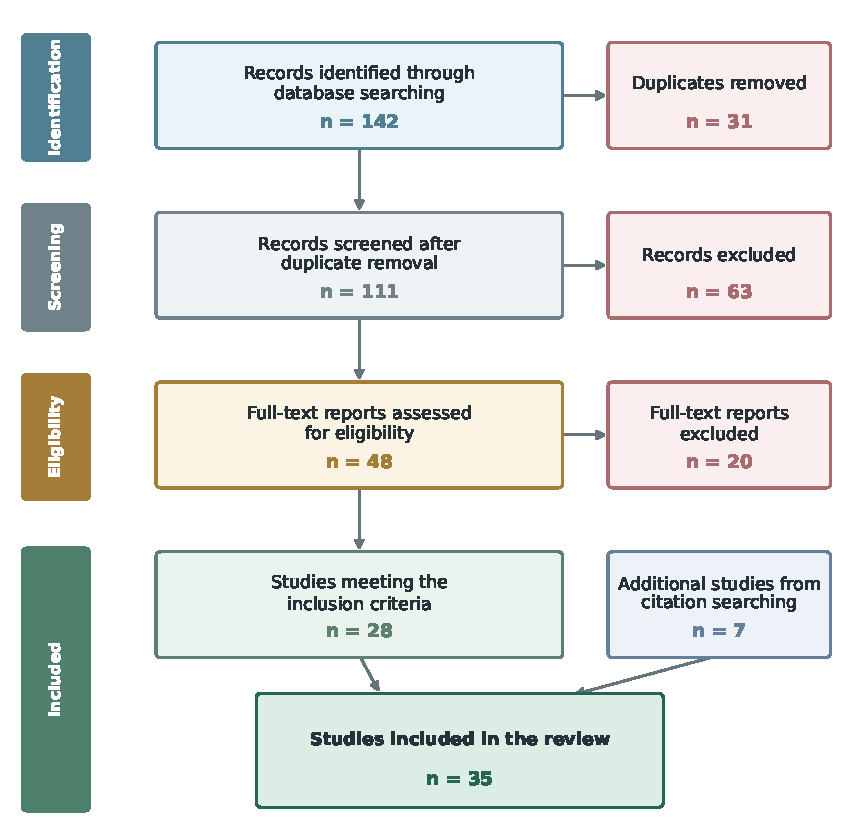
\includegraphics[width=0.88\textwidth]{prisma_literature_flow.pdf}
\caption[PRISMA literature-selection flow diagram]{PRISMA flow diagram
summarising the selection of the 35 publications included in the review.}
\label{fig:prisma-flow}
\end{figure}

The selected studies cover cardiac MRI data and segmentation, statistical shape
models, learned 3D reconstruction, and wall-thickness measurement. The next
section relates these areas to the specific problem of recovering paired LV
surfaces from sparse contours.

% ============================================================
\section{Technical Background}
\label{sec:literature-background}
% ============================================================

\noindent
This section introduces the geometric concepts needed to compare the reviewed
methods. It separates what is observed in cardiac MRI from what a reconstruction
method must infer, and then contrasts the main ways in which the resulting 3D
anatomy can be represented.

\subsection{From SAX slices to paired LV surfaces}
\label{subsec:sax-paired-surfaces}

\noindent
Cine cardiac MRI records the heart at several points in the cardiac cycle.
End-diastole (ED) corresponds approximately to the phase at which the LV cavity
is largest, while end-systole (ES) corresponds to its smallest state. These two
phases provide a compact description of ventricular contraction and are the
phases labelled in commonly used benchmarks such as ACDC
\parencite{bernard2018acdc}.

In a short-axis acquisition, each image plane cuts across the ventricular long
axis. The in-plane anatomy is sampled in detail, but consecutive planes are
separated by a larger distance. The resulting stack is therefore anisotropic:
spatial resolution depends on direction
\parencite{petitjean2011segmentationreview}. A segmentation can identify the
visible myocardium on every acquired plane, but it does not directly observe
how the boundary bends, tapers, or changes between those planes.

Two contours are needed on each slice. The endocardial contour bounds the blood
cavity, while the epicardial contour bounds the outer myocardium. In three
dimensions these contours become two nested surfaces. Their relationship is as
important as either surface alone: an intersection, reversal, or local collapse
would imply an invalid myocardial wall. Reconstructing the surfaces separately
can therefore create a plausible cavity and outer boundary while still failing
to produce a valid wall between them.

The reconstruction problem is underdetermined because many smooth surfaces can
pass through the same contour rings. A method must decide how much shape is
inferred from the observations and how much is supplied by a prior learned from
other hearts. Strong smoothing gives stable surfaces but may remove real
regional variation. A strong population prior can fill large gaps but may pull
an abnormal ventricle towards common anatomy. Conversely, fitting every contour
closely can preserve the observations while reproducing segmentation noise or
creating abrupt changes between slices.

For this reason, reconstruction quality has several dimensions. The surface
should remain close to the observed anatomy, form a closed geometry where a
volume is required, preserve patient-specific differences, and maintain a valid
wall at both cardiac phases. No single overlap or surface-distance metric tests
all of these properties. The evaluation must combine geometric distance,
volumetric agreement, topology, and the stability of measurements derived from
the wall.

\subsection{Representations of three-dimensional anatomy}
\label{subsec:geometry-representations}

\noindent
Three-dimensional cardiac anatomy can be stored as a voxel volume, an explicit
surface mesh, or an implicit field. A voxel volume follows the image grid and is
convenient for segmentation, overlap measures, and distance transforms. Its
spatial detail is limited by the grid resolution, however, and interpolation is
still needed where the acquired slices are far apart.

A triangular mesh represents the boundary directly through vertices, edges, and
faces. It supports surface distances, enclosed-volume calculations, regional
partitioning, and colour maps of local measurements. Meshes with consistent
topology and vertex correspondence are also useful for population statistics.
Their quality depends on how the vertices are connected and distributed, and
operations such as smoothing, remeshing, or hole repair can alter the geometry
being evaluated.

Statistical shape models provide one way to generate corresponded meshes. They
describe each anatomy as a mean shape plus weighted population modes
\parencite{cootes1995asm,heimann2009ssmreview}. This gives a compact and
controllable shape space, but it links the output to the topology and variation
present in the atlas. An SSM is therefore well suited to supplying a geometric
prior or synthetic training examples, but it is not an independent observation
of a new patient's anatomy.

An implicit representation defines geometry through a function evaluated at
continuous coordinates. An occupancy field predicts whether a point is inside
or outside the anatomy, whereas a signed distance function also represents the
distance to the boundary \parencite{deepsdf2019,occupancynetworks2019}. The
surface is the zero-level set of this function and can be extracted on a grid
with an algorithm such as Marching Cubes
\parencite{lorensen1987marchingcubes}. Because the function is continuous, the
extraction resolution is not fixed by an output template.

For a true signed distance function, the gradient magnitude is one almost
everywhere away from singular points. Eikonal regularisation encourages a neural
field to retain this property even when dense distance targets are unavailable
\parencite{gropp2020igr}. Fourier coordinate features can improve the recovery
of finer spatial variation that a standard multilayer perceptron tends to smooth
\parencite{tancik2020fourierfeatures}. These properties make implicit fields
attractive for interpolating sparse contours, although the final mesh still
depends on field quality, extraction resolution, and post-processing.

When two nested surfaces are needed, two independent implicit functions do not
guarantee their ordering. A coupled representation can instead define one
surface relative to the other through a positive separation. This changes the
problem from predicting two unrelated boundaries to predicting a reference
surface and a constrained wall. The reviewed literature provides the individual
elements of this approach, but their integration for phase-conditioned LV
reconstruction is the specific gap examined later in this chapter.

% ============================================================
\section{Related Work}
\label{sec:related-work}
% ============================================================

\noindent
This section synthesises the reviewed literature, organised by thematic area.

\subsection{Cardiac MRI segmentation and datasets}
\label{subsec:cardiac-segmentation}

\noindent
Short-axis (SAX) cine MRI is the standard protocol for left-ventricle (LV)
evaluation, producing 2D slices perpendicular to the long axis with high
in-plane resolution (1--2~mm) but large inter-slice gaps (6--10~mm)
\parencite{petitjean2011segmentationreview,cerqueira2002segmentation}. This
anisotropic acquisition creates the central reconstruction problem: the
observed contours are detailed within each slice, but the geometry between
slices, especially near the apex and base, must be inferred. The AHA 17-segment
model provides a common anatomical frame for reporting the resulting regional
measurements \parencite{cerqueira2002segmentation}.

Modern segmentation networks can identify endocardial and epicardial boundaries
reliably on the acquired slices. U-Net established the encoder--decoder pattern
used by many medical segmentation systems, while nnU-Net showed that much of
their configuration can be adapted automatically to a dataset
\parencite{ronneberger2015unet,isensee2021nnunet}. These methods improve the
quality of the observed contours, but they do not by themselves determine the
unobserved 3D surface between slices.

The distinction between segmentation and reconstruction is important here.
U-Net combines broad image context with fine spatial detail through skip
connections, making it suitable for delineating thin myocardial boundaries.
The self-configuring design of nnU-Net reduces the need to tune preprocessing,
network scale, and post-processing separately for each dataset. Both approaches
still optimise agreement on sampled image planes. A high slice-wise overlap can
therefore coexist with an uncertain surface between planes, because no image
evidence directly constrains that part of the anatomy.

The ACDC benchmark provides expert ED and ES labels across several clinical
groups, including normal and hypertrophic ventricles
\parencite{bernard2018acdc}. The M\&Ms challenge extends this setting across
centres, scanner vendors, and diseases, showing that performance on one source
does not guarantee reliable transfer to another \parencite{campello2021mnms}.
Together, these datasets support model development on varied clinical images
while also exposing the limits of generalisation.

ACDC contains 100 cases divided among five diagnostic groups and supplies
labels at the two phases with the largest functional contrast, ED and ES. It is
therefore useful for studying whether a reconstruction changes appropriately
with cardiac phase and whether abnormal shape is retained. M\&Ms contains 375
studies from several centres and scanner vendors. Its principal lesson is that
variation in acquisition can be as important as variation in anatomy: a method
that performs well on one source may lose accuracy on unseen data. This limits
claims based on any single evaluation cohort and supports the use of varied
clinical data during fine-tuning.

At population scale, the UK Biobank provides a large and standardised cardiac
MRI resource \parencite{sudlow2015ukbiobank}. Automated segmentation of this
cohort has enabled large anatomical studies and statistical atlases
\parencite{bai2018automated}. These resources establish two complementary forms
of evidence used in this thesis: slice-wise clinical observations and
population-level knowledge of plausible 3D cardiac shape.

The two forms are not interchangeable. Clinical labels retain subject-specific
and pathological variation, but their through-plane geometry is only indirectly
observed. A population atlas supplies complete and consistent surfaces, but it
reflects the cohort and processing choices from which it was built. Combining
them can reduce the weakness of either source alone, provided that the atlas is
used as a prior rather than treated as patient-specific ground truth.

\subsection{Statistical shape models}
\label{subsec:ssm-review}

\noindent
Statistical Shape Models (SSMs) encode anatomical variability by aligning a
training population to point-to-point correspondence and applying PCA to extract
the dominant modes of variation \parencite{cootes1995asm,heimann2009ssmreview}.
They provide a compact description of plausible shape, but their quality depends
on anatomical correspondence, alignment, and the diversity of the population
used to construct them.

In a point-distribution model, the corresponding coordinates of each training
shape are concatenated into one vector. Principal component analysis separates
the mean anatomy from directions of population variation, and a new shape is
formed by weighting those directions \parencite{cootes1995asm}. Restricting the
weights to the range represented in the training population provides a practical
plausibility constraint. This compact representation is useful when complete
meshes are scarce, although it assumes that the main variation can be described
within a linear shape space.

Cardiac SSMs have progressed from multi-object ventricular models to large
population atlases. Dense correspondence allows coupled structures to be
represented consistently across subjects \parencite{frangi2002cardiacssm}, while
the UK Digital Heart Project atlas captures population variation in ventricular
shape and motion \parencite{bai2015biventricularatlas}. This makes an SSM more
than an average heart: its modes describe coordinated changes in size,
proportion, apical form, and regional curvature.

The move from single structures to coupled cardiac models is relevant because
the geometry of one surface is not independent of its neighbours.
\textcite{frangi2002cardiacssm} used non-rigid registration to establish dense
correspondence in a multi-object model, allowing related ventricular structures
to vary together. \textcite{bai2015biventricularatlas} then constructed a
large-scale atlas from more than one thousand cardiac MRI studies. The first 50
modes represented about 90\% of the observed shape variance, showing that a
moderate latent space can retain substantial population variation while keeping
all generated meshes in correspondence.

Those modes can support both population analysis and disease studies. Previous
work has related cardiac shape variation to hypertrophic remodelling, normal
anatomical diversity, and myocardial infarction
\parencite{demarvao2014atlas,medrano2014lvshapevariation,suinesiaputra2018infarctchallenge}.
The important point for reconstruction is that a shape prior can preserve
structured variation that a simple smooth template would remove.

These studies also show why global volume alone is insufficient.
\textcite{demarvao2014atlas} found shape patterns associated with hypertrophic
remodelling that were not captured fully by conventional volumetric indices.
\textcite{medrano2014lvshapevariation} identified modes related to size,
eccentricity, apical form, and regional curvature in a large multi-ethnic
cohort. SSM-derived features have also been used to distinguish infarcted from
healthy ventricles \parencite{suinesiaputra2018infarctchallenge}. A useful
reconstruction prior must therefore retain regional variation rather than force
every case towards one mean geometry.

SSMs therefore have two useful roles. They can constrain reconstruction to a
learned shape space, or they can generate synthetic geometries by sampling that
space \parencite{heimann2009ssmreview,khalafvand2018lvflowssm}. This thesis uses
the second role for pre-training: the SSM supplies complete, plausible meshes
before the model is fine-tuned on sparse contours from clinical images.

Synthetic sampling increases the amount of complete geometric supervision, but
it cannot introduce anatomy absent from the source atlas. It may also
under-represent rare or severe pathology when the retained PCA modes favour
common variation. The real-data fine-tuning stage is therefore essential: it
allows the reconstruction to move beyond the synthetic prior while retaining
the surface continuity learned from complete meshes. This division of roles is
the main reason for combining SSM and clinical data rather than choosing one of
them as the sole training source.

\subsection{Deep learning models for 3D shape reconstruction}
\label{subsec:dl-reconstruction-review}

\noindent
Classical reconstruction methods interpolate between segmented SAX slices using
splines or deformable surfaces. Their result depends on the sampled contours and
the assumptions imposed between slices, particularly near the apex and base
\parencite{petitjean2011segmentationreview,heimann2009ssmreview}.
Simple interpolation can preserve the observations but may introduce staircase
artefacts, whereas restrictive parametric surfaces can smooth away individual
shape. Learned reconstruction methods address this trade-off through two main
families: template deformation and implicit field prediction.

Template methods learn to displace the vertices of a fixed mesh. Pixel2Mesh and
Pose2Mesh demonstrate that graph-based deformation can recover dense geometry
from sparse image or landmark evidence
\parencite{wang2018pixel2mesh,choi2020pose2mesh}. In cardiac applications, fixed
correspondence is valuable for population analysis and regional measurement
\parencite{bai2015biventricularatlas,suinesiaputra2014collaborative,beetz2021cardiacshape}.
The trade-off is that the output remains tied to the topology and resolution of
the chosen template.

Implicit Neural Representations (INRs) take a different approach. Rather than
deforming a template, they encode geometry as a continuous function whose
zero-level set defines the surface. DeepSDF represents a shape class through a
latent-conditioned signed distance function, while Occupancy Networks learn a
continuous inside--outside decision
\parencite{deepsdf2019,occupancynetworks2019}. Both separate the learned geometry
from a fixed output mesh and allow a surface to be extracted at a chosen
resolution, commonly with Marching Cubes
\parencite{lorensen1987marchingcubes}.

Recent cardiac work shows why implicit representations are useful when MRI
slices are far apart. In a SAX scan, the detailed shape of the ventricle is
observed within each slice, but less information is available between slices.
\textcite{bras2026anisotropy} addressed this anisotropy problem with a neural
implicit representation that reconstructs the left and right ventricles,
including the endocardial and epicardial boundaries of the LV myocardium. The
study is closely related to the problem considered here because both approaches
seek continuous cardiac shape from incomplete observations. Br{\'a}s et al.
use image data directly, whereas this thesis isolates the geometric problem by
using segmented contour points.

\textcite{muffoletto2026nihc} also reconstruct three-dimensional cardiac shape
from sparse segmentations with a neural implicit representation. Their method
uses a learned biventricular shape prior and includes both SAX and long-axis
views. It is therefore broader than the LV-focused SDF reconstruction considered
here. The study does not report a public dataset or code release, which limits
its direct reproducibility and comparison with this work.

Two techniques are critical for applying INRs to thin cardiac structures where
high-frequency geometric detail must be preserved. Fourier features reduce the
low-frequency bias of standard multilayer perceptrons, and Eikonal regularisation
encourages the learned field to behave like a signed distance function
\parencite{tancik2020fourierfeatures,gropp2020igr}. These ideas support smooth
interpolation without abandoning local surface detail.

Recent cardiac INRs also model motion across the cardiac and respiratory cycles
\parencite{kunz2024fourierinr,quillien2025sensorfree,wang2025dvrnemf,tian2026mocoinr}.
Their main goal is temporally coherent image or volume reconstruction. The
present work has a narrower geometric goal: it conditions paired surface
reconstruction on ED or ES and then measures the wall between those surfaces.

For encoding unordered input observations such as SAX contour points, the
PointNet architecture \parencite{qi2017pointnet} provides a
permutation-invariant encoder via shared MLPs followed by symmetric max-pooling.
This is a natural match for SAX contours because their point ordering should not
change the reconstructed anatomy. A PointNet-style encoder can therefore reduce
the observed contour set to a latent description used by an implicit decoder.

\subsection{Wall-thickness measurement techniques}
\label{subsec:thickness-review}

\noindent
Myocardial wall thickness is a primary clinical biomarker for cardiac
remodelling. \textcite{grossman1974wallthickness} demonstrated that wall
thickness is a principal determinant of left-ventricular diastolic stiffness,
with hypertrophied ventricles exhibiting markedly elevated stiffness
proportional to end-diastolic wall thickness. More recently,
\textcite{huelnhagen2017t2wallthickness} showed at 7.0T MRI that wall thickness
correlates with tissue transverse relaxation properties, confirming its value as
a non-invasive surrogate for myocardial tissue characterisation. The AHA 17-segment model
\parencite{cerqueira2002segmentation} provides the standard framework for
reporting regional thickness values.

The accuracy of wall-thickness measurement depends critically on the quality of
the underlying surface reconstruction, as any smoothing or geometric artefact
propagates directly into the thickness estimate. The literature describes
five families of measurement methods, each with distinct trade-offs.

The simplest approach uses nearest-neighbour distance: for each endocardial
vertex, a KD-tree identifies the closest epicardial point, yielding a
measurement in $O(N \log M)$ time. Its runtime depends on mesh size and the
implementation. This method can provide a lower bound on the true
transmural thickness because it ignores the anatomical direction of measurement
--- the nearest point may lie tangentially rather than across the wall.

Ray-based methods address this limitation by casting a ray from each endocardial
vertex along its surface normal until it intersects the epicardium. The
intersection is computed via the M\"{o}ller--Trumbore algorithm, accelerated with
a Bounding Volume Hierarchy (BVH) to $O(\log F)$ per query. This approach
measures transmurally but is sensitive to normal noise: a slightly rotated
normal can produce a spurious long or short ray. The Shape Diameter Function
variant improves robustness by casting a cone of $K$ rays (typically $K{=}7$) at
a half-angle of $30^{\circ}$ around the normal and reporting the median intersection
distance, effectively filtering outlier hits caused by local mesh irregularities.

Volumetric methods operate on voxelised representations. The Euclidean Distance
Transform (EDT) computes, for each myocardial voxel, the distance to the nearest
boundary, and the sum of the endocardial and epicardial distance fields
approximates local thickness ($t = D_{\mathrm{endo}} + D_{\mathrm{epi}}$). This
estimate is exact for planar parallel boundaries but can be biased in curved
regions because the nearest-boundary directions do not necessarily follow a
common transmural path. The method is computationally efficient ($O(V)$ via the
Saito--Toriwaki algorithm) but limited by voxel resolution.

Partial differential equation (PDE)-based methods are widely used for transmural thickness estimation.
\textcite{jones2000laplace} solved Laplace's equation between the two tissue
boundaries and used the resulting non-intersecting field lines to establish
corresponding paths. Thickness is obtained from the path length between the
boundaries along these streamlines. \textcite{yezzi2003thickness} formulated an
Eulerian PDE method that computes distances propagated from both boundaries
along the Laplacian field. Their sum gives the local tissue thickness.

Finally, mesh-based regularised correspondence methods combine an initial
geometric estimate (normal projection or nearest neighbour) with iterative
Laplacian smoothing on the mesh connectivity graph. At each iteration, each
vertex's thickness is updated as a weighted average of its neighbours, anchored
to the initial estimate. This produces spatially smooth thickness maps suitable
for bullseye visualisation, at the cost of potentially attenuating real local
thickness variation if the smoothing parameter is set too aggressively.

\subsection{Summary and research gap}
\label{subsec:research-gap}

\noindent
The reviewed literature shows that each component of the LV analysis pipeline is
well-studied in isolation: deep learning gives accurate slice-wise segmentation,
SSMs encode population-level shape priors, implicit representations provide
continuous surface modelling, and multiple wall-thickness algorithms exist.
To the best of our knowledge, however, limited work integrates these components
into a single pipeline for the specific setting addressed in this thesis. The
combination that appears to be missing is a method
that encodes sparse SAX contour points, decodes paired endocardial and
epicardial surfaces as implicit signed distance fields, conditions the
reconstruction on cardiac phase, constrains the wall offset to stay positive,
and trains jointly on real clinical data and SSM-derived synthetic
samples. This is useful because the wall can then be measured everywhere on a
continuous surface instead of only on the acquired slices. This gap motivates
the approach described in the remaining chapters.

% ============================================================
% !TeX root = ../main.tex
%  Chapter 3 — Methodology
% ============================================================
\chapter{Methodology}
\label{ch:methodology}

\noindent This chapter describes the proposed approach to address the
research questions stated in \cref{sec:research-questions}.

\section{Overview}
\label{sec:method-overview}
\noindent
% TODO: high-level overview of the approach. A diagram (TikZ) helps here.

\section{System Architecture}
\label{sec:architecture}
\noindent
% TODO: describe the architecture and main components.

% Example figure placeholder:
% \begin{figure}[htbp]
%   \centering
%   \includegraphics[width=0.8\textwidth]{architecture-diagram}
%   \caption{Overview of the proposed system architecture.}
%   \label{fig:architecture}
% \end{figure}

\section{Components}
\label{sec:components}

\subsection{Component A}
\label{subsec:component-a}
\noindent
% TODO

\subsection{Component B}
\label{subsec:component-b}
\noindent
% TODO

\section{Implementation Details}
\label{sec:implementation}
\noindent
% TODO: technology stack, libraries, key design decisions.

% Example code listing:
% \begin{lstlisting}[language=Python, caption={Example function.}, label={lst:example}]
% def example():
%     pass
% \end{lstlisting}

% ============================================================
% !TeX root = ../main.tex
%  Chapter 4 — Results and Evaluation
% ============================================================
\chapter{Results and Evaluation}
\label{ch:results}

\noindent This chapter presents the experimental evaluation of the approach
described in \cref{ch:methodology}.

\section{Experimental Setup}
\label{sec:setup}
\noindent
We evaluate the final CardioSDF model, obtained by pre-training on the synthetic
SSM meshes and then fine-tuning on the real end-diastolic (ED) and end-systolic
(ES) data, as described in \cref{ch:methodology}. The datasets, quality gates,
and patient-level splits are reported in \cref{subsec:dataset-composition}; all
numbers below are computed on the held-out test partitions, which contain no
patient seen during training. Two questions guide the evaluation: how faithfully
the model reconstructs the LV surfaces from sparse contours, and how the analytic
wall thickness it produces compares with independent measurement algorithms
applied to the same geometry.

\subsection{Metrics}
\label{subsec:metrics}
\noindent
Reconstruction quality is measured with four quantities. The \emph{Chamfer
distance} averages, for every reconstructed vertex, the distance to the nearest
ground-truth surface point and vice versa, reported separately for the
endocardium and the epicardium in millimetres; smaller is better. The
\emph{slice residual} is the mean absolute signed-distance value at the input
contour points, and measures how closely the reconstructed surface passes
through the observed short-axis (SAX) rings, again in millimetres. The
\emph{watertight rate} is the fraction of reconstructed meshes that form a
closed surface with no holes. The \emph{volume ratio} is the reconstructed
cavity or wall volume divided by its ground-truth value, so that a value of one
indicates no systematic over- or under-estimation.

Wall thickness is summarised by its mean, its dispersion (standard deviation),
and its 5th and 95th percentiles across the myocardial surface, all in
millimetres. These percentiles describe the thin apical and thick basal
extremes without being distorted by isolated outliers.

\subsection{Baselines}
\label{subsec:baselines}
\noindent
Because no paired ground-truth 3D mesh exists for the clinical scans (see
\cref{subsec:missing-ground-truth}), the reconstruction is compared against the
derived meshes built from the segmentations, and the analytic wall thickness is
compared against the four measurement algorithms selected in
\cref{subsec:thickness-methods}: the Laplace field method, the Yezzi--Prince
method, the SDF cone-ray method, and the Euclidean Distance Transform (EDT)
boundary sum kept as a volumetric baseline. As an external plausibility anchor,
we also report the mean wall thickness obtained directly from the input
segmentation.

\section{Results}
\label{sec:results}
\noindent
This section reports first the geometric quality of the reconstruction and then
the wall-thickness measurements obtained from the reconstructed geometry.

\subsection{Reconstruction Quality}
\label{subsec:reconstruction-quality}
\noindent
\Cref{tab:reconstruction-quality} summarises the reconstruction accuracy on the
test set. The endocardial and epicardial surfaces are recovered with a mean
Chamfer distance of $1.12$~mm and $1.17$~mm respectively, which is close to the
$1.0$~mm isotropic resolution of the prepared data and therefore near the limit
of what the derived meshes can resolve. The mean slice residual of $0.57$~mm
shows that the reconstructed surfaces pass through the observed SAX contours
with sub-millimetre agreement, confirming that the model honours its input. The
cavity and wall volumes are reproduced almost exactly, with volume ratios of
$1.00$ for the endocardium and $1.02$ for the epicardium.

Every reconstructed mesh is watertight, for both the endocardium and the
epicardium. This is a direct consequence of reading the surfaces as zero-level
sets of a continuous signed-distance field rather than assembling them from
per-slice contours, and it holds without any mesh repair, hole filling, or cap
synthesis. The monotone-epi coupling also guarantees a strictly positive wall:
the analytic thickness never collapses to zero, with a 5th percentile of
$2.33$~mm that stays well above the enforced floor.

\begin{table}[htbp]
  \centering
  \caption{Reconstruction quality of the final CardioSDF model on the test set.
    Chamfer distance and slice residual are in millimetres; the volume ratio is
    dimensionless with an ideal value of one.}
  \label{tab:reconstruction-quality}
  \begin{tabular}{l c}
    \toprule
    Metric & Value \\
    \midrule
    Endocardium Chamfer distance (mm) & 1.12 \\
    Epicardium Chamfer distance (mm)  & 1.17 \\
    Slice residual (mm)               & 0.57 \\
    Endocardium volume ratio          & 1.00 \\
    Epicardium volume ratio           & 1.02 \\
    Watertight rate (endocardium)     & 100\% \\
    Watertight rate (epicardium)      & 100\% \\
    \bottomrule
  \end{tabular}
\end{table}

\subsection{Wall-Thickness Measurement}
\label{subsec:wall-thickness-results}
\noindent
The analytic wall thickness read directly from the decoder has a mean of
$5.31 \pm 0.41$~mm across the test set, with a 5th percentile of $2.33$~mm and a
95th percentile of $6.67$~mm. These values fall within the normal range for the
LV myocardium and are consistent with the four independent algorithms applied to
the same reconstructed surfaces.

\Cref{tab:wall-thickness-results} lists the mean, standard deviation, and 5th and
95th percentiles for each of the four selected methods, and
\cref{fig:wall-thickness-comparison} shows the same comparison graphically. The
three transmural estimators agree to within roughly one millimetre of the mean:
the Laplace field reports $5.08$~mm, the SDF cone-ray method $5.47$~mm, and the
Yezzi--Prince method $4.30$~mm. The EDT boundary sum returns a lower mean of
$3.58$~mm, as expected for a voxel-based estimator that measures the shortest
transmural distance and therefore reads low in curved regions; it is retained
only as a baseline. For reference, the mean wall thickness measured directly from
the input segmentation is $3.61$~mm, and a plain nearest-neighbour measurement on
the model surface gives $4.55$~mm, so the surface-based and field-based
estimators bracket the segmentation reference from above, as expected when the
reconstruction fills in a smooth, complete wall rather than a slice-limited one.

\begin{table}[htbp]
  \centering
  \caption{Wall-thickness statistics for the four selected methods, computed on
    the CardioSDF-generated LV geometry. All values are in millimetres.}
  \label{tab:wall-thickness-results}
  \begin{tabular}{l c c c c}
    \toprule
    Method & Mean & Std. & $p_{5}$ & $p_{95}$ \\
    \midrule
    Laplace field (state of the art) & 5.08 & 1.70 & 2.92 & 8.62 \\
    Yezzi--Prince (recent)           & 4.30 & 1.43 & 0.96 & 5.80 \\
    SDF cone rays (promising)        & 5.47 & 1.15 & 3.25 & 7.16 \\
    \addlinespace
    EDT boundary sum (baseline)      & 3.58 & 0.86 & 1.49 & 4.81 \\
    \bottomrule
  \end{tabular}
\end{table}

\begin{figure}[htbp]
  \centering
  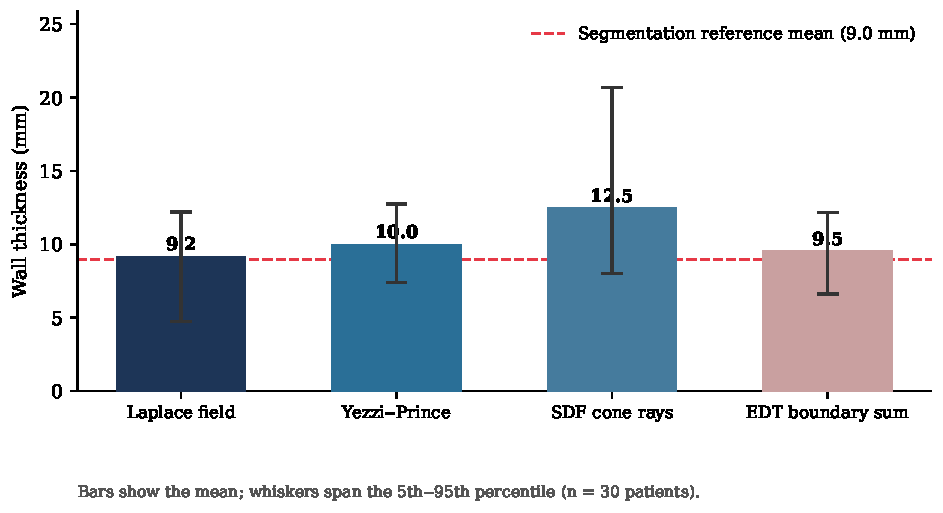
\includegraphics[width=0.9\textwidth]{wall_thickness_methods_comparison}
  \caption{Mean wall thickness of the four selected methods on the reconstructed
    LV geometry, with whiskers spanning the 5th to 95th percentile. The dashed
    line marks the mean wall thickness measured directly from the input
    segmentation.}
  \label{fig:wall-thickness-comparison}
\end{figure}

\section{Discussion}
\label{sec:discussion}
\noindent
The results support the two central design choices of CardioSDF. First, encoding
the LV as a signed-distance field yields watertight surfaces in every test case
without any post-processing, which removes the mesh-repair heuristics that a
contour-stacking pipeline would otherwise require. Second, the monotone-epi
coupling delivers a wall that is positive everywhere, so the analytic thickness
is usable as a measurement rather than merely a by-product: its mean of
$5.31$~mm and its percentile range agree with the established Laplace field and
with the SDF cone-ray estimator to within about one millimetre.

The spread between methods is informative rather than contradictory. Field-based
transmural estimators and surface-based ray estimators measure thickness along
slightly different paths, and the EDT baseline reads systematically lower because
straight-line voxel distances underestimate thickness where the wall curves. The
agreement of the three transmural methods, together with the sub-millimetre slice
residual and near-unit volume ratios, indicates that the reconstructed geometry
is both accurate at the observed slices and plausible between them, which is
precisely where sparse SAX acquisitions provide no direct evidence.

\section{Threats to Validity}
\label{sec:threats}
\noindent
The most important limitation concerns the ground truth. The reconstruction is
evaluated against meshes \emph{derived} from the segmentations, not against
independently acquired 3D surfaces, so the Chamfer distances measure agreement
with a derived target rather than with true anatomy. For the same reason, the
wall-thickness comparison is an inter-method and reproducibility study on shared
geometry, not a clinical validation: without expert manual wall-thickness
measurements, the thesis can claim an objective and locally resolved
computational framework, but not the replacement of clinical measurement
protocols.

Several further factors bound the external validity of the results. The real
data come from two public collections (ACDC and M\&Ms-2), and the ES test
partition is small, so per-phase estimates carry more uncertainty than the ED
ones. The wall-thickness percentiles depend on the AHA orientation and on the
$96^3$ inference grid, both of which introduce discretisation effects that a
finer grid or an alternative anatomical frame could shift. Finally, the synthetic
epicardium used during pre-training is a geometric construction rather than a
measured surface, which the fine-tuning stage on real data is designed to
correct but cannot fully rule out as a residual prior.

% ============================================================
% !TeX root = ../main.tex
%  Chapter 5 — Conclusions
% ============================================================
\chapter{Conclusions}
\label{ch:conclusions}

\noindent This chapter summarises the contributions,
revisits the research questions, and outlines directions for future work.

\section{Summary}
\label{sec:summary}
\noindent
% TODO: summarise the work in one or two paragraphs.

\section{Revisiting the Research Questions}
\label{sec:revisit-rqs}
\noindent
% TODO: answer each research question stated in \cref{sec:research-questions}.

\section{Contributions}
\label{sec:contributions-summary}
\noindent
% TODO: list the contributions again, this time backed by the evidence
% presented in \cref{ch:results}.

\section{Limitations}
\label{sec:limitations}
\noindent
% TODO: honestly state the limitations of the work.

\section{Future Work}
\label{sec:future-work}
\noindent
% TODO: suggest concrete directions for future research and development.


% ============================================================
\backmatter

\renewcommand{\bibname}{References}
\printbibliography[heading=bibintoc, title={References}]

\appendix
% ============================================================
% !TeX root = ../main.tex
%  Appendix A — Supplementary Methodological Details
% ============================================================
\chapter{Supplementary Methodological Details}
\label{app:supplementary-methods}

\noindent
This appendix records supporting methodological material that would otherwise
repeat information established in the main text.

\section{Training data streams}
\label{sec:appendix-training-streams}
\noindent
All three training streams use the shared cache representation described in
\cref{subsec:training-cache-representation}. The table below provides a compact
reference for their source, cardiac phase, and role in the two-stage training
procedure.

\begin{table}[H]
	\centering
	\caption{Data streams sharing the cache schema and their role in training.}
	\label{tab:method-datasets}
	\small
	\renewcommand{\arraystretch}{1.12}
	\begin{tabular}{p{0.18\textwidth} p{0.10\textwidth} p{0.29\textwidth} p{0.31\textwidth}}
		\toprule
		Stream & Phase & Source & Training role \\
		\midrule
		Synthetic SSM & ED & UK Digital Heart Project LV SSM & Pre-training to establish a geometric shape prior \\
		Real MRI & ED & ACDC, M\&Ms, and M\&Ms-2 & Fine-tuning on patient-specific diastolic anatomy \\
		Real MRI & ES & ACDC, M\&Ms, and M\&Ms-2 & Fine-tuning on systolic anatomy with phase conditioning \\
		\bottomrule
	\end{tabular}
\end{table}


\end{document}
